\documentclass[11pt]{article}
\usepackage{titlesec}

\setcounter{secnumdepth}{4}

\parindent 0px % no automatic indentation

\usepackage{amsmath,amssymb,amstext,amsthm,amsfonts}
\usepackage{float}
\usepackage[shortlabels]{enumitem}
\usepackage[a4paper,lmargin={2cm},rmargin={2cm},tmargin={2.5cm},bmargin = {2.5cm},headheight = {4cm}]{geometry}

\usepackage[utf8]{inputenc}
\usepackage[T1]{fontenc}
%\usepackage[ngerman]{babel}
\usepackage{lmodern}
\usepackage{color}
\usepackage{xcolor}
\usepackage{colortbl}
\usepackage{graphicx}
\usepackage{listings}
\usepackage{xspace}
\usepackage{empheq}
\usepackage{mdframed}
\usepackage{changepage}
%\usepackage{hanging}
\usepackage{romanbar}
\usepackage{mathtools}
\usepackage[hidelinks]{hyperref}

\usepackage[headsepline]{scrlayer-scrpage} 
\pagestyle{scrheadings} 
\usepackage{titling}
\usepackage{cancel}
\usepackage{booktabs}

\usepackage{algpseudocode}

\usepackage{listings}
\usepackage{xcolor} % Optional, for coloring code

\usepackage[ruled,vlined]{algorithm2e}

\lstset{ 
  language=C,                     % the language of the code
  basicstyle=\ttfamily,           % the size of the fonts that are used for the code
  keywordstyle=\color{blue},      % keywords are color blue
  commentstyle=\color{gray},      % comments are color gray
  stringstyle=\color{red},        % strings are color red
  numbers=left,                   % where to put the line-numbers; possible values are (none, left, right)
  numberstyle=\tiny\color{gray},  % the style that is used for the line-numbers
  stepnumber=1,                   % the step between two line-numbers. If it's 1, each line will be numbered
  numbersep=5pt,                  % how far the line-numbers are from the code
  backgroundcolor=\color{white},  % choose the background color. You must add \usepackage{color}
  showspaces=false,               % show spaces adding particular underscores
  showstringspaces=false,         % underline spaces within strings
  showtabs=false,                 % show tabs within strings adding particular underscores
  frame=single,                   % adds a frame around the code
  tabsize=4,                      % sets default tabsize to 4 spaces
  captionpos=b,                   % sets the caption-position to bottom
  breaklines=true,                % sets automatic line breaking
  breakatwhitespace=false,        % sets if automatic breaks should only happen at whitespace
  escapeinside={\%*}{*)}          % if you want to add LaTeX within your code
}


\setlist[itemize]{itemsep=0pt, topsep=2pt}
\setlist[enumerate]{itemsep=0pt, topsep=2pt}

\pagestyle{plain}

% MACROS
\newcommand{\ind}{\perp\!\!\!\!\perp} 


\title{Informatics II}
\author{Michael Sigg}
\date{\today}

\ohead{\theauthor}
\ihead{Informatics II, Spring 24}



\begin{document}
\maketitle
\tableofcontents

\newpage

\section{Introduction, Sorting, Recursion}
\subsection{Algorithms}

\subsection{Sorting}
Problem specification
\begin{itemize}
    \item Input: s sequence of $n$ numbers $A=[a_1,a_2,\cdots,a_n]$
    \item Output: a permutation (reordering) $]b_1,b_2,\cdots,b_n]$ of the input sequence such that $b_1 \leq b_2 \leq \cdots \leq b_n$
\end{itemize}

\subsubsection{Bubble Sort}
Rough idea:
\begin{itemize}
    \item Scan sequence and swap unsorted adjacent elements
    \item Repeat the procedure until sequence is actually sorted
\end{itemize}

\begin{center}
\begin{minipage}{0.4\textwidth}
\begin{algorithm}[H]
\caption{BubbleSort(A)}
\For{$i = n$ \KwTo $2$}{
    \For{$j = 2$ \KwTo $i$}{
        \If{$A[j] < A[j-1]$}{
            $t = A[j]$\;
            $A[j] = A[j-1]$\;
            $A[j-1] = t$\;
        }
    }
}
\end{algorithm}
\end{minipage}
\end{center}

Basic properties: 
\begin{itemize}
    \item Number of comparisons:
    \[
    C = \sum_{i=2}^n(i-1)=\sum_{i=1}^{n-1}=\frac{(n-1)n}{2}=\frac{n^2-n}{2}
    \]
    \item Number of moves:
    \begin{align*}
        &Mmin=0 \\
        &Mmax = \sum_{i=2}^n 3(i-1) = \frac{3n(n-1)}{2} = \frac{3n^2-3n}{2}
    \end{align*}
\end{itemize}



\subsubsection{Selection Sort}
Rough idea: 
\begin{itemize}
    \item Select smallest element and swap with 1st element
    \item Repeat the procedure on remaining unsorted sequence
\end{itemize}

\begin{center}
\begin{minipage}{0.6\textwidth} % Adjust the width as needed
\centering % Center the content within the minipage
\begin{algorithm}[H]
\caption{SelectionSort(A)}
\For{$i = 1$ \KwTo $n-1$}{
    $k = i$\;
    \For{$j = i+1$ \KwTo $n$}{
        \If{$A[j] < A[k]$}{
            $k = j$\;
        }
    }
    exchange $A[i]$ and $A[k]$\;
}
\end{algorithm}
\end{minipage}
\end{center}

Basic properties:
\begin{itemize}
    \item Number of comparisons:
    \[
    C= \sum_{i=1}^{n-1} i = \frac{n^2-n}{2}
    \]
    \item Number of moves: (3 because 1 swap is 3 operations) \[
    M= \sum_{i=1}^{n-1} 3=3(n-1)=3n-3
    \]
\end{itemize}

\subsubsection{Insertion Sort}
Rough idea:
\begin{itemize}
    \item Take first element and consider it as (sorted) sequence
    \item Continue taking elements and inserting into right place
\end{itemize}

\begin{center}
\begin{minipage}{0.6\textwidth} % Adjust the width as needed
\centering % Center the content within the minipage
\begin{algorithm}[H]
\caption{InsertionSort(A)}
\For{$i = 2$ \KwTo $n$}{
    $j = i-1$\;
    $t=A[i]$\;
    \While{$j \geq 1 \land t < A[j]$}{
        $A[j+1] = A[j]$\;
        $j=j-1$\;
    }
   $ A[j+1]=t$\;
}
\end{algorithm}
\end{minipage}
\end{center}

Basic properties:
\begin{itemize}
    \item Number of comparisons:
    \begin{align*}
        &Cmin = \sum_{i=2}^n 1 = n-1 \\
        &Cmax = \sum_{i=2}^n (i-1)=\frac{n^2-n}{2}
    \end{align*}
    \item Number of moves:
    \begin{align*}
        &Mmin = \sum_{i=2}^n 2 = 2(n-1) = 2n-2 \\
        &Mmax = \sum_{i=2}^n (i+1)=\frac{n^2 + 3n-4}{2}
    \end{align*}
\end{itemize}

\subsection{Recursion}

\subsection{Summary}
\begin{itemize}
    \item Algorithmic problem:
    \begin{itemize}
        \item An algorithm transforms input data into output data
        \item Precisely specify \textbf{input} and \textbf{output}; consider special cases; work out representative examples
        \item A first step is to come up with a simple plan
        \item Split or revise complex plans until they get simple
    \end{itemize}
    \item Sorting algorithms
    \begin{itemize}
        \item A classical and representative algorithmic problem
        \item Initialization and conditions in loop are important
        \item Make sure you get details of loops \textbf{correct by design}. Avoid trial and error
    \end{itemize}
    \item Recursive algorithms
    \begin{itemize}
        \item Recursion is an important algorithmic technique
        \item Practice the design of recursive algorithms
        \item Consider \textbf{special cases}: termination, the first couple of recursive calls
    \end{itemize}
\end{itemize}

\section{Complexity and Correctness}
\subsection{Algorithmic Complexity}
\subsubsection{Efficiency}
Analysis of algorithms
\begin{itemize}
    \item Predicting the resources that the algorithm requires
    \begin{itemize}
        \item Resources in terms of time: running time
        \item Resources in terms of space: memory usage
    \end{itemize}
\end{itemize}

\noindent
\textbf{\underline{Example: Runtime of Insertion Sort}} \\
\bigskip

\begin{figure}[H]
    \centering
    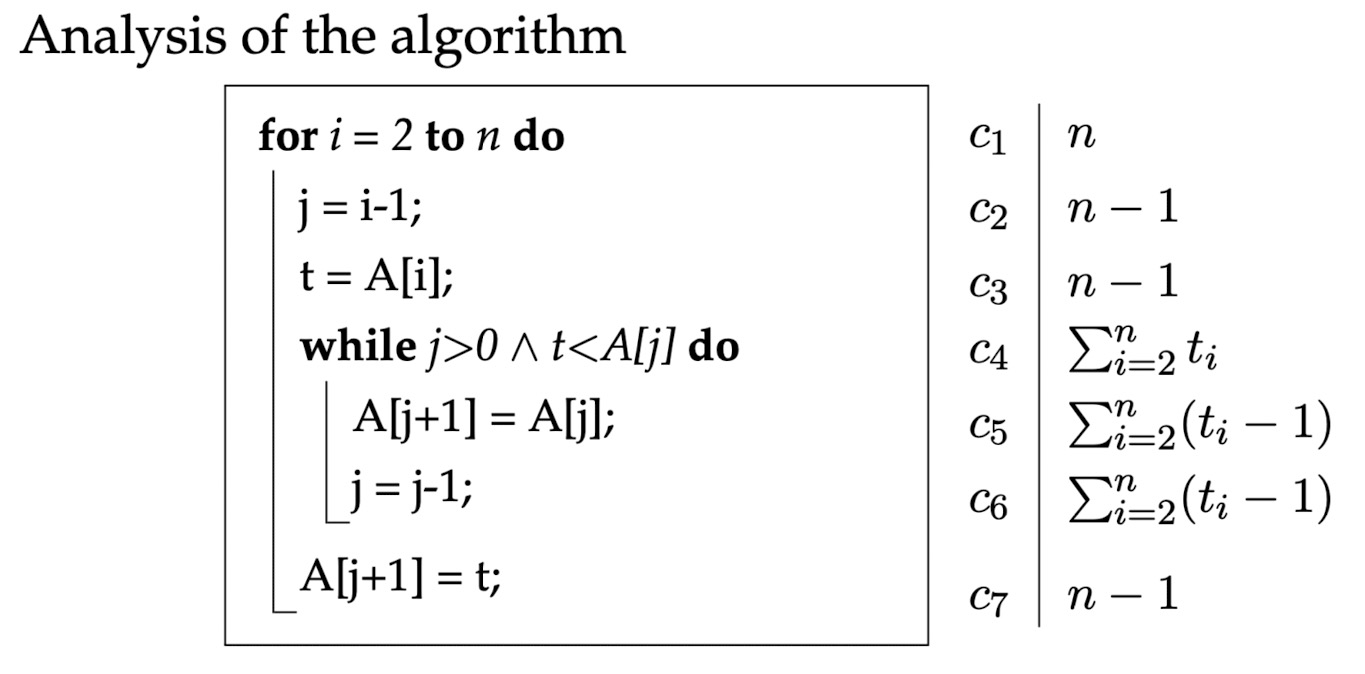
\includegraphics[width=0.5\linewidth]{images/Screenshot 2024-05-24 at 13.57.47.jpg}
\end{figure}

Exact running time: Sum of products (cost, times) \[
T(n)=c_1n + c_2(n-1)+c_3(n-1)+c_4\sum_{i=2}^n t_i + c_5 \sum_{i=2}^n (t_i-1) +c_6 \sum_{i=2}^n (t_i-1)+c_7(n-1)
\]
$\Rightarrow$ Running time as a function of the input size $n$ \\

\textbf{Best case} running time: (Already sorted; $t_i=1$)
\begin{align*}
    T(n)&=c_1n +(c_2+c_3+c_4+c_7)(n-1) \\
    &= \underbrace{(c_1+c_2+c_3+c_4+c_7)}_{a}n -\underbrace{(c_2+c_3+c_4+c_7)}_{b} \\
    &=an+b
\end{align*}
\textbf{Worst case} running time: (Reverse order; $t_i=i$)
\begin{align*}
    T(n)&=c_1n+(c_2+c_3+c_7)(n-1)+c_4\left (\frac{n(n+1)}{2} -1 \right) + (c_5+c_6) \frac{(n-1)n}{2} \\
    &= an^2+bn+c
\end{align*}
\begin{itemize}
    \item In depth explanations of terms:
    \begin{itemize}
        \item $n$ = amount of times the outer loop condition is being checked 
        \item $n-1$ = times the outer loop runs
        \item $\frac{n(n+1)}{2}-1$ = the amount the inner loop condition is being checked
        \begin{itemize}
            \item In the first iteration, we have to compare $n$ elements, thus make $n-1$ comparisons $\Rightarrow$ Inner loop runs $n-1$ times and condition is being checked one time more, thus $n$ times
            \item But as the outer loop runs from $i=2$, the loop $i=1$ is never run. This mean the inner condition is being checked: $n+(n-1)+\cdots+2$ times 
            \item In order to calculate sum of the arithmetic series $\sum_{i=2}^n i$, we have to look at $\sum_{i=1}^n i-1$, thus we get $\frac{n(n+1)}{2} - 1$. [\ref{ARSeries}]
        \end{itemize}
    \end{itemize}
\end{itemize}

\subsubsection{Best, Worst and Average Case: Concluding Remarks}
\begin{itemize}
    \item Often, counting the number of iterations of the core (innermost) part is sufficient
    \begin{itemize}
        \item No distinction between comparisons, assignments, etc.
        \item Means that each of them has roughly the same cost
        \item Does provide results with good/adequate precision
    \end{itemize}
    \item In certain cases the cost of a specific operation may dominate all other costs
    \begin{itemize}
        \item Example: disk I/O versus RAM operations
    \end{itemize}
\end{itemize}

\noindent
\textbf{\underline{Example: Runtime of Binary Search}} \\
\bigskip

\begin{center}
\begin{minipage}{0.6\textwidth}
\begin{algorithm}[H]
\caption{LinSearch(A, v)}
\textbf{Input:} sequence $A[1..n]$ of length $n$, value $v$ \\
\textbf{Output:} either index $i$ such that $v = A[i]$ or $\text{NIL}$ \\
$i = 1$ \\
\While{$i \leq n \land A[i] \neq v$} {
    $i = i + 1$\;}
\If{$i \leq n$} {
     \textbf{return} $i$\;
     }
\Else {
     \textbf{return} $\text{NIL}$\;
     }
\end{algorithm}
\end{minipage}
\end{center}
\begin{itemize}
    \item Running times of Linear Search:
    \begin{itemize}
    \item Worst case: $n$
    \item Average case: $\frac{n}{2}$
    \item Best case: 0
\end{itemize}
\end{itemize}


\begin{center}
\begin{minipage}{0.6\textwidth}
\begin{algorithm}[H]
\caption{BinSearch1(A, v)}
\KwIn{sequence $A[1..n]$ of length $n$, value $v$}
\KwOut{either index $i$ such that $v == A[i]$ or \text{NIL}}
$l = 1$; $r = n$\;
$m = \lfloor (l + r) / 2 \rfloor$\;
\While{$l \leq r$ $\land$ $v \neq A[m]$}{
    \uIf{$v < A[m]$}{
        $r = m - 1$\;
    }
    \Else{
        $l = m + 1$\;
    }
    $m = \lfloor (l + r) / 2 \rfloor$\;
}
\If{$l \leq r$} {
    \Return $m$\;
}
\Else{
    \Return \text{NIL}\;
}
\end{algorithm}
\end{minipage}

\end{center}

Analysis of algorithm:
\begin{itemize}
    \item How many times is the loop executed?
    \begin{itemize}
        \item $log_2n$ - better than linear $n$
    \end{itemize}
\end{itemize}

\subsection{Correctness}

Pre/post-conditions:
\begin{itemize}
    \item \textbf{Assertion}: statement about the state of execution
    \item To prove partial correctness one associates a number of assertions with specific checkpoints in the algorithm
    \item \textbf{Preconditions}: assertions that must be valid before the execution of an algorithm or a subroutine (input)
    \item \textbf{Postconditions}: assertions that must be valid after the execution of an algorithm or a subroutine (output)
\end{itemize}
Loop invariants:
\begin{itemize}
    \item To show correctness of loop statements
    \item \textbf{Invariants}: assertions that are valid any time they are reached
    \item One must show three things about loop invariants 
    \begin{enumerate}
        \item Initialization: it is true before the first iteration
        \item Maintenance: if it is true before an iteration then it is true after that iteration
        \item Termination: when the loop terminates, it gives a useful property that helps to show that the algorithm is correct 
    \end{enumerate}
\end{itemize}

\subsubsection{Correctness of Binary Search}

Invariant: 
\begin{itemize}
    \item $\forall i \in [1..l-1]:v>A[i]$, and
    \item $\forall i \in [r+1..n]:y < A[i]$
    \item In words: elements to the left (right) of $l$ ($r$) are smaller (larger) than v 
\end{itemize}

\textbf{Initialization}: $l=1,r=n$ \\
The invariant holds because there are no elements to the left or right of $l$ and $r$ respectively.
\begin{itemize}
    \item $l=1$ yields $\forall i \in [1..0]:A[i] < v$. This holds since the range [1..0] is empty
    \item $r=n$ yields $\forall i \in [n+1..n]:A[i]>v$. This holds since the range [n+1..n] is empty
\end{itemize}
\textbf{Maintenance}: $l,r,m = \lfloor (l+r)/2 \rfloor $\\
Two cases:
\begin{itemize}
    \item We have $A[m]\neq v, A[m] > v, r=m-1 $, A is sorted. This implies $\forall k \in [r+1..n]:A[k]>v$
    \item We have $A[m] \neq v, A[m] < v, l=m+1 $, A is sorted. This implies $\forall k \in [1..l-1]:A[k]<v $
\end{itemize}

\textbf{Termination}: $l,r,l \leq r$\\
Two cases:
\begin{itemize}
    \item $l=m+1$ allows to conclude $\lfloor(l+r)/2\rfloor +1 >l $
    \item $r=m-1$ allows to conclude $\lfloor(l+r)/2\rfloor -1 < r $
\end{itemize}
Thus, the range gets smaller during each iteration and the loop will terminate when $l\leq r$ no longer holds

\subsubsection{Correctness of Insertion Sort}
Outer loop:
\begin{itemize}
    \item $A[1..i-1]$ is sorted
    \item $A[1..i-1[ \in A^{orig}$ 
\end{itemize}
Inner loop:
\begin{itemize}
    \item $A[i..j],t,A[j+1...i-1]$
    \item $t<A[k]$ for $j+1\leq k \leq i-1$
    \item $A[i..j] \circ A[j+1...i-1]$ sorted
\end{itemize}

\textbf{Initialization}
\begin{itemize}
    \item $i=2$: invariant holds; $A[1..1]$ is trivially sorted 
    \item $j= i-1: A[1..i-1],t,A[i..i-1],t=A[i]$
    \item[] $A[i..i-1]$ is empty (and thus trivially sorted)
    \item[] $A[1..i-1]$ is sorted (invariant of outer loop) 
\end{itemize}

\textbf{Maintenance}
\begin{itemize}
    \item $A[1..i-1]$ is sorted + insert $A[i]$ implies $A[1..i]$ is sorted
    \item $A[1..j-1],t,A[j,j+1..i-1]$ satisfies condition since
    \item[] $A[j]>t $ and $A[1..i-1] $ is sorted
\end{itemize}

\textbf{Termination}
\begin{itemize}
    \item outer loop: $i=n+1$ and $A[1..n]$ is sorted
    \item $A[j]\leq t:A[1..j],t,A[j+1..i-1]=A[1..i] $ is sorted
    \item $j=0: A[t,1..i-1] = A[1..i]$ is sorted
\end{itemize}

\subsection{Asymptotic Complexity}

Asymptotic Analysis
\begin{itemize}
    \item Goal: simplify the analysis of running time
    \item Approach: getting rid of unnecessary details
    \item Fundamental concern: how the running time increases with the size of the input in the limit
\end{itemize}

\subsubsection{Order of Growth}
\textbf{Big-$O$ notation:}
\begin{itemize}
    \item Asymptotic upper bound
    \item Used for \textbf{worst-case analysis}
    \item $f(n)$ and $g(n)$ are function over non-negative integers
    \item $f(n)= O(g(n))$ if and only if there exists constants $c>0$ and $n_0>0$ such that $f(n9 \leq cg(n)$ for $n\geq n_0$
    \item Example proofs:
    \begin{itemize}
        \item $2^{n+1} = O(2^n)$
        \begin{align*}
            2^{n+1} &\leq c\cdot 2^n \\
            2\cdot 2^n &\leq c\cdot 2^n\\
            2&\leq c\\
            \text{holds for } c&\geq 2
        \end{align*}
    \end{itemize}
\end{itemize}
\textbf{Big-$\Omega$ notation}
\begin{itemize}
    \item Asymptotic lower bound
    \item Used for best-case analysis
    \item $f(n) =\Omega(g(n))$ if and only if there exist constants $c>0$ and $n_0>0$ such that $cg(n) \leq f(n) $ for $n\geq n_0$
\end{itemize}

\textbf{Big-$\Theta$ notation}
\begin{itemize}
    \item Asymptotic tight bound
    \item $f(n)= \Theta(g(n))$ if and only if there exist constants $c_1 >0$, $c_2>0$, and $n_0>0$ such that $c_1g(n)\leq f(n) \leq c_2g(n)$ for $n \geq n_0$
    \item $f(n) = \Theta(g(n))$ iff $f(n) = O(g(n))$ and $f(n) = \Omega(g(n))$
\end{itemize}

Useful analogy:
\begin{itemize}
    \item $f(n)=O(g(n)) \quad \leftrightarrow f \leq g $
    \item $f(n)=o(g(n)) \quad \leftrightarrow f < g$
    \item $f(n)=\Omega(g(n)) \quad \leftrightarrow f \geq g$
    \item $f(n)=\omega (g(n)) \quad \leftrightarrow f>g$
    \item $f(n) = \Theta(g(n)) \quad \leftrightarrow f=g$
\end{itemize}


\subsection{Special case analysis}
Basic approach for checking the correctness of a program with special case analysis:
\begin{itemize}
    \item Consider all possible extreme cases
    \item Make sure the solution works in these cases
    \item Problem is reduced to identifying all the special cases 
\end{itemize}

Special cases:
\begin{itemize}
    \item Data structure: empty, single element, completely filled, duplicates, etc.
    \item Particular values, border of domain: Zero, empty string, negative numbers, etc.
    \item Calling of functions (procedures): entering function, termination of function
    \item Control and loop statements: start of loop, end of loop, 1st iteration
\end{itemize}

\section{Divide and Conquer, Recurrences}

\subsection{Divide and Conquer}

Designing algorithms
\begin{itemize}
    \item Recursive algorithms: divide-and-conquer approach
    \item Principle: if problem size is small enough to be solved trivially then solve it; else
    \begin{enumerate}
        \item \textbf{Divide} problem into a number of subproblems
        \item \textbf{Conquer} subproblems by solving them recursively
        \item \textbf{Combine} solutions of the subproblems into solution for the original problem
    \end{enumerate}
\end{itemize}

\subsubsection{Merge Sort}
Rough idea:
\begin{itemize}
    \item To sort an $n$-element sequence proceed as follows
    \begin{itemize}
        \item \textbf{Divide}: divide the sequence into two $n/2$-element sequences
        \item \textbf{Conquer}: sort the two sequences recursively using merge sort
        \item \textbf{Combine}: merge the two sorted sequences to produce the solution
    \end{itemize}
    \item Recursion stops when the sequence has length 1
\end{itemize}

\begin{center}
\begin{minipage}{0.6\textwidth} % Adjust the width as needed
\centering % Center the content within the minipage
\begin{algorithm}[H]
\caption{MergeSort(A,l,r)}
\KwIn{array $A[l..r]$}
\KwOut{permuted array $A[l..r]$ that is sorted in increasing order}
\If{$l<r$} {
$m= \lfloor (l+r)/2 \rfloor$\;
MergeSort(A,l,m)\;
MergeSort(A,m+1,r)\;
Merge(A,l,r,m)\;
}
\end{algorithm}
\end{minipage}
\end{center}

\begin{center}
\begin{minipage}{0.6\textwidth} % Adjust the width as needed
\centering % Center the content within the minipage
\begin{algorithm}[H]
\caption{Merge(A,l,r,m)}
\KwIn{array A; indexes l,r, and m from MergeSort}
\KwOut{$A[l,,r]$ is sorted in increasing order}
\For{$i = l$ \KwTo $m$}{
    $B[i] = A[i]$\;
}
\For{$i = m+1$ \KwTo $r$}{
    $B[r+m-i+1] = A[i]$\;
}
$i = l$; $j = r$\;
\For{$k = l$ \KwTo $r$}{
    \uIf{$B[i] < B[j]$}{
        $A[k] = B[i]$\;
        $i = i + 1$\;
    }
    \Else{
        $A[k] = B[j]$\;
        $j = j - 1$\;
    }
}
\end{algorithm}
\end{minipage}
\end{center}

Running time may be calculate via several methods. See below.


\subsection{Recurrences}

Running times of algorithms with recursive calls can be described using recurrences.\\

\subsubsection{Repeated (backward) substitution}
\begin{itemize}
    \item Not a strict formal proof
    \item Procedure
    \begin{itemize}
        \item Substitute, expand, substitute, etc.
        \item Observe a pattern and determine the expression after the $i$-th substitution
        \item Find out what the highest value of $i$ should be to get the base case of the recurrence
        \item Insert the cost of the base case and the expression for $i$ into the observed expression
    \end{itemize}
\end{itemize}

\underline{Example:} Merge Sort
\begin{itemize}
    \item For $n>1$, let $T(n)=2T(n/2)+cn$
    \item Apply repeated substitution
    \begin{align*}
        T(n) &= 2\textcolor{red}{T(n/2)} + cn && \text{(substitute)} \\   
        &= 2(\textcolor{red}{2T(n/4)+cn/2})+cn &&\text{(expand)}\\
        &= 4\textcolor{blue}{T(n/4)} + 2cn &&\text{(substitute)} \\
        &= 4(\textcolor{blue}{2T(n/8)+cn/4})+2cn &&\text{(expand)}\\
        &= 8T(n/8)+3cn &&\text{{find pattern}} \\
        &= 2^iT(n/2^{i})+icn
    \end{align*}
    \item Calculate max $i$:
    \begin{align*}
        \frac{n}{2^{i}} &= 1\\
        \Rightarrow i &= \log_2 n = i_{max}
    \end{align*}
    \item Insert into pattern:\[
    2^{\log_2 n} T(n/2^{\log_2 n}) + cn \log_2 n= nT(1)+cn \log_2 n = \boxed{\Theta(n \log_2 n)}
    \]
\end{itemize}

\subsubsection{Substitution method}
Basic methodology
\begin{enumerate}
    \item Guess the form of the solution 
    \item User induction to prove the solution
\end{enumerate}

\underline{Example:} \\

Proof by induction
\begin{itemize}
    \item Need to show that $\overbrace{T(n)\leq cn^3}^\text{hypothesis}$ for $T(n)=4T(n/2)+n$
    \begin{align*}
        T(n) &= 4T(n/2)+n &&\text{(recurrence)}\\
        &\leq 4c(n/2)^3 + n &&\text{(inductive hyp.)}\\
        &=cn^3/2 + n &&\text{(simplification)}\\
        &= cn^3 -\underbrace{(cn^3/2-n)}_{\geq 0} &&\text{(rearrangement)}\\
        &\leq cn^3 &&\text{(for $c\geq2, n\geq1$)}
    \end{align*}
    \item It follows that $T(n)=O(n^3)$
\end{itemize}
Getting a tighter bound 
\begin{itemize}
    \item Underlying problem: $T(n)\leq cn^2$ does not work in the inductive proof (leads to contradiction), thus try to rewrite as \[
    T(n)=O(n^2) = cn^2 + (\text{something positive})
    \]\item Solution: strengthen hypothesis for inductive proof \[
    T(n) \leq (\text{answer you want})- (\text{something positive})
    \]
        \item Show that $T(n)\leq cn^2-dn$ for $T(n)=4T(n/2)+n$
    \begin{align*}
        T(n) &= 4\textcolor{red}{T(n/2)}+n &&\text{(recurrence)}\\
        &\leq 4(\textcolor{red}{c(n/2)^2-dn/2})+n &&\text{(inductive hyp.)}\\
        &=cn^2-2dn + n &&\text{(simplification)}\\
        &= cn^2 - dn -\underbrace{(dn-n)}_{\geq 0 \text{ for } d\geq 1} &&\text{(rearrangement)}\\
        &\leq cn^2 - dn &&\text{(for $d\geq1$)}
    \end{align*}
    \item It thus follows that $T(n)=O(n^2)$
\end{itemize}


\subsubsection{Recursion trees}
Basic methodology
\begin{itemize}
    \item A recursion tree is a convenient way to visualize what happens when a recurrence is iterated
    \item Good for guessing asymptotic solutions to recurrences
    \item Example: $T(n)=T(n/4)+T(n/2)+n^2$
    \begin{itemize}
        \item Tree with $n^2$ at the top, as this is the largest term
    \end{itemize}
\end{itemize}
\underline{Example:}
\begin{itemize}
    \item Show that $T(n)\leq cn^2$ for $T(n)=T(n/2) + T(n/4) + n^2$
    \begin{align*}
        T(n)&= T(n/2)+T(n/4)+n^2 &&\text{(recurrence)}\\
        &\leq c(n/2)^2 + c(n/4)^2 + n^2 &&\text{(inductive hyp.)}\\
        &= 5cn^2 /16 +n^2 &&\text{(simplification)} \\
        &= cn^2 - 11cn^2/16 +n^2 &&\text{(rearrangement)}\\
        &\leq cn^2 &&\text{(for $c\geq 16/11$)}
    \end{align*}
    \item It thus follows that $T(n)=O(n^2)$
\end{itemize}

\subsubsection{Master method}
To solve a class of recurrences that have the form \[
T(n) + a T(n/b)+f(n)
\]
\begin{itemize}
    \item Assumptions: 
    \begin{itemize}
        \item $a\geq 1$
        \item $b>1$, and
        \item $f(n)$ asymptotically positive
    \end{itemize}
    \item $T(n)$ describes running time of a divide-and-conquer algorithm 
    \begin{itemize}
        \item $a$ subproblems of size $n/b$ are solved recursively, each in time $T(n/b)$
        \item $f(n)$ is the cost of dividing the problem and combining the solutions
    \end{itemize}
    \item Iterating the recurrence (expanding the tree) yields: 
    \begin{align*}
        T(n) &= f(n) + a T(n/b) \\
        &= f(n) + af(n/b) + a^2T(n/b^2) \\
        &=f(n) + af(n/b) + a^2f(n/b^2) + \cdots + \underbrace{a^{\log_n n-1}f(n/b^{\log_b n-1}) + a^{\log_b n }T(1)}_\text{leaves} \\
        &= \sum_{i=0}^{\log_b n-1} a^i f(n/b^i) + \Theta(n^{\log_b a})
    \end{align*}
\end{itemize}

Underlying intuitions
\begin{itemize}
    \item Three possible cases
    \begin{enumerate}
        \item Running time dominated by the cost at the leaves (case 1)
        \item Running time evenly distributed throughout tree (case 2)
        \item Running time dominated by the cost at the root (case 3)
    \end{enumerate}
    \item Solve recurrence by identifying dominant term
    \item In each case compare $f(n)$ with $n^{\log_b a}$
\end{itemize}


\textbf{\underline{Master theorem, case 1:}} 
\begin{itemize}
    \item $f(n)=O(n^{\log_ba-\epsilon})$ for some constant $\epsilon>0$
    \begin{itemize}
        \item $f(n)$ grows polynomially slower than $n^{\log_b a}$ (by factor $n^\epsilon$)
    \end{itemize}
    \item The work at the leaves dominates: $T(n)= \Theta(n^{\log_ba})$
\end{itemize}


 
\textbf{\underline{Master theorem, case 2:}} 
\begin{itemize}
    \item $f(n)=\Theta(n^{\log_b a})$ (i.e., $f(n)$ and $n^{\log_b a}$ are asymptotically the same)
    \item The work is evenly distributed: $T(n)=\Theta(n^{\log_b a} \log_b n)$
\end{itemize}



\textbf{\underline{Master theorem, case 3:}} 
\begin{itemize}
    \item $f(n)=\Omega(n^{\log_b a + \epsilon})$ for some constant $\epsilon>0$
    \begin{itemize}
        \item $f(n)$ grows polynomially faster than $n^{\log_b a}$ (by factor $n^\epsilon$)
        \item Regularity: $\exists c < 1, \exists n_0 > 0, \forall n > n_0, (af(n/b) \leq cf(n))$
    \end{itemize}
    \item The work at the root dominates: $T(n) = \Theta(f(n))$
\end{itemize}

\textbf{\underline{General Strategy:}}
\begin{itemize}
    \item Extract $a,b$ and $f(n)$ from given recurrence
    \item Determine $n^{\log_b a}$; asymptotically compare it with $f(n)$
    \item Determine and apply the appropriate master theorem case
    \item There are recurrences where no Master theorem case applies
\end{itemize}


\section{Heap Sort, Quick Sort}
\subsection{Heap Sort}

\subsubsection{Binary trees}

\begin{minipage}{0.6\textwidth}
    \begin{itemize}
        \item Each node may have a left or a right child (or both)
        \item Each node has at most one parent 
        \item The root has no parent
        \item A leaf has no children
        \end{itemize}
        \end{minipage}
        \begin{minipage}{0.4\textwidth}
            \begin{figure}[H]
                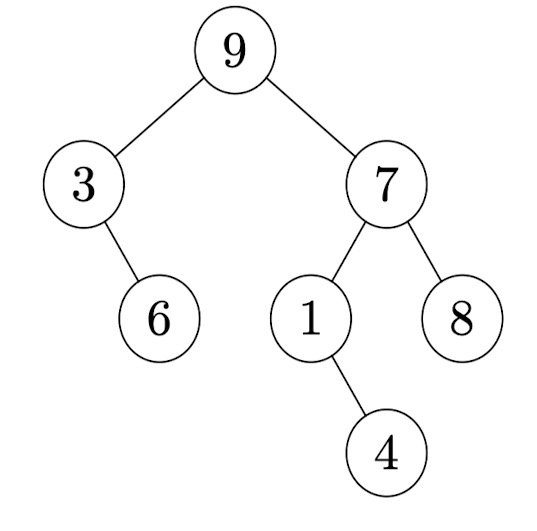
\includegraphics[width=.5\linewidth]{images/Screenshot 2024-05-30 at 14.59.56.jpg}
            \end{figure}
        \end{minipage}
\begin{itemize}
    \item The depth (level) of a node $x$ is the length of the path from the root to $x$
    \item The height of a node $x$ is the length from the longest path from $x$ to a leaf
    \item The height of a tree is the height of its root
    \item The right (left) subtree of a node $x$ is the tree rooted at the right (left) child of $x$
\end{itemize}

\subsubsection{Complete trees}
\begin{itemize}
    \item A \textbf{complete binary tree} is a binary tree where
    \begin{itemize}
        \item all the leaves have the same depth
        \item all internal nodes have two children
    \end{itemize}
        \item A \textbf{nearly complete binary tree} is a binary tree where
        \begin{itemize}
            \item all levels of non-maximal depth $d$ are full (have $2^d$ nodes)
            \item all the leaves with maximal depth are as far left as possible
        \end{itemize}
\end{itemize}

\subsubsection{Heap}
Definition of heap:
\begin{itemize}
    \item A binary tree is a (binary) \textbf{heap} if and only if 
    \begin{itemize}
        \item it is a nearly complete binary tree and, 
        \item each node is greater than or equal to all its children
    \end{itemize}
\end{itemize}
Heaps and arrays are closely related (can use array to represent a heap): 
\begin{figure}[H]
    \centering
    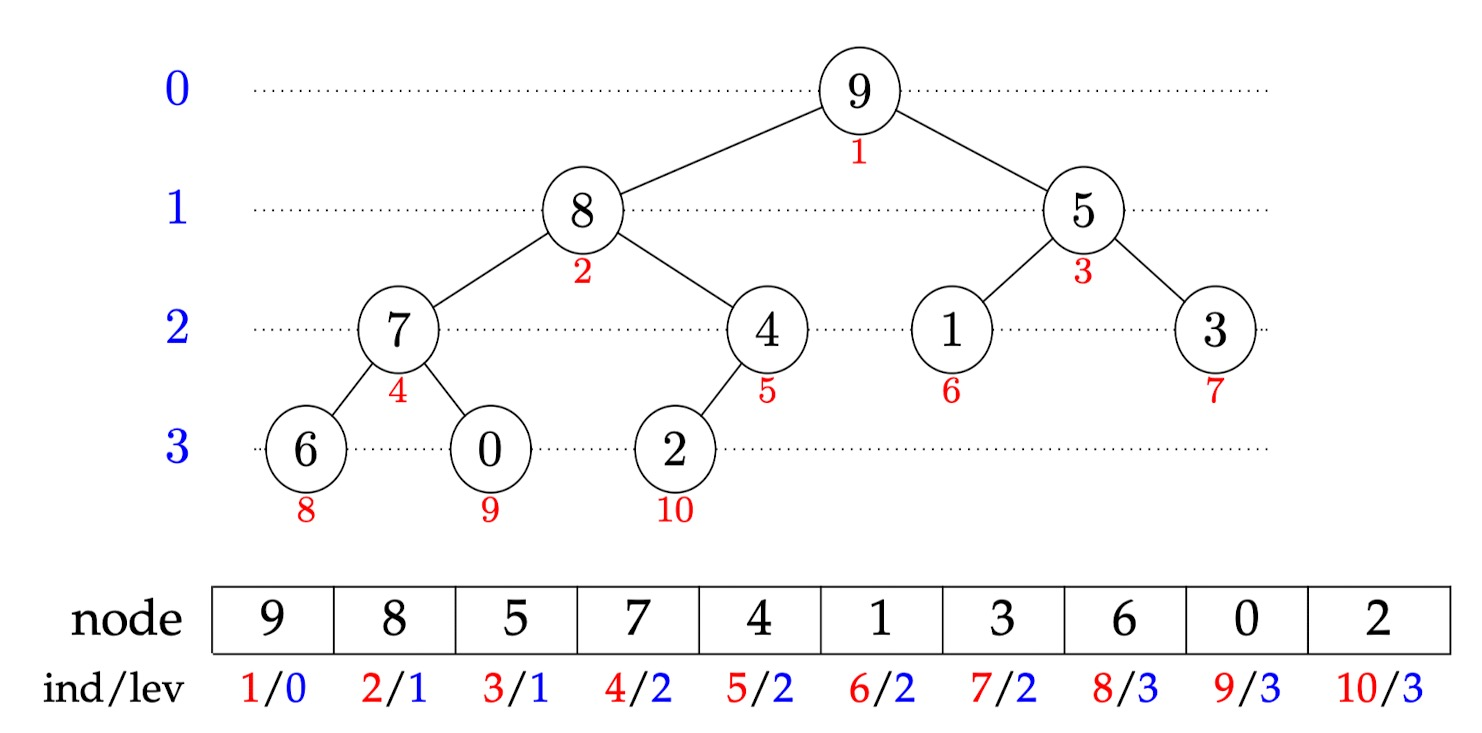
\includegraphics[width=0.75\linewidth]{images/Screenshot 2024-05-30 at 15.11.16.jpg}
\end{figure}

Fundamental properties
\begin{itemize}
    \item Let $i$ be a node index
    \item Heap property: $A[parent(i)]\geq A[i]$
    \item A binary heap can be efficiently stored as an array (because it is a nearly complete binary tree)
    \item Finding parent, left child, and right child:
    \begin{figure}[H]
        \centering
        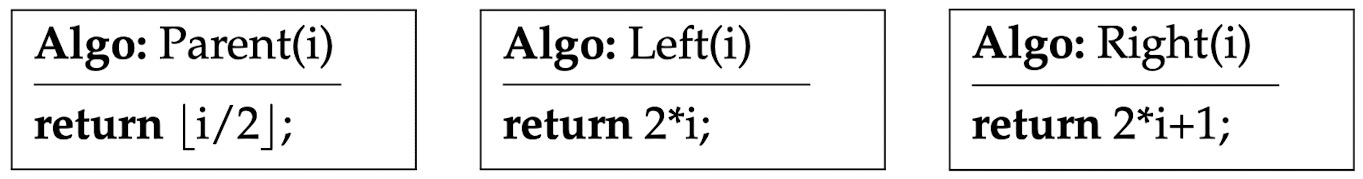
\includegraphics[width=0.5\linewidth]{images/Screenshot 2024-05-30 at 15.13.23.jpg}
    \end{figure}
    \item A heap where the largest (smallest) element is at the root is a max-heap (min-heap)
    \item A binary heap can be exploited for sorting arrays
\end{itemize}

\subsubsection{Heapify}
\begin{itemize}
    \item Input: index $i$ in array $A$, number $s$ of heap elements
    \item Binary trees rooted at \texttt{left}($i$) and \texttt{right}($i$) are binary heaps
    \item $A[i]$ may be smaller than its children, thus violating the heap property
    \item \texttt{heapify}($A,i,s$) transforms the binary tree rooted at $i$ into a binary heap
    \item Strategy: move $A[i]$ down the heap until the heap property is satisfied again
\end{itemize}

\begin{center}
\begin{minipage}{0.6\textwidth} % Adjust the width as needed
\centering % Center the content within the minipage
\begin{algorithm}[H]
\caption{Heapify(A,i,s)}
m = i\;
l = Left(i)\;
r = Right(i)\;
\If{$l<s \land A[l]>A[m]$} {
m = 1\;
}
\If{$r\leq s \land A[r]>A[m]$} {
m = r\;
}
\If{$i\neq m$} {
exchange $A[i]$ and $A[m]$\;
Heapify(A,m,s)\;
}
\end{algorithm}
\end{minipage}
\end{center}

Running time:
\begin{itemize}
    \item The running time of heapify on a subtree of size $n$ rooted at $i$ includes time to 
    \begin{itemize}
        \item determine relationship between elements: $\Theta(1)$
        \item run heapify on a subtree rooted at one of $i$'s children
    \end{itemize}
    \item $2n/3$ is the worst case size of the subtree (half filled bottom level) and thus \[
    T(n) \leq T(2n/3)+\Theta(1), \text{ i.e., } T(n)=O(\log_2 n)
    \]
\end{itemize}

\subsection{Building A Heap}
\begin{itemize}
    \item Convert an array $A$ with $n$ elements into a heap
    \item Note that the elements in $A \left[ \lfloor n/2 + 1 \cdots n \right]$ are 1-element heaps
\end{itemize}

\begin{center}
\begin{minipage}{0.6\textwidth} % Adjust the width as needed
\centering % Center the content within the minipage
\begin{algorithm}[H]
\caption{BuildHeap(A,n)}
\For{$i=\lfloor n/2 \rfloor$ \KwTo 1}{Heapify(A,i,n)\;}
\end{algorithm}
\end{minipage}
\end{center}

Correctness:
\begin{itemize}
    \item Loop invariant: all trees rooted at $m>i$ are heaps
\end{itemize}
Running time:
\begin{itemize}
    \item There are $O(n)$ calls to heapify and so $T(n) = O(n \log_2 n)$
    \item Not an asymptotically tight bound 
    \item Tight bound - Intuition:
    \begin{itemize}
        \item An $n$-element binary heap has height $\log_2 n$
        \item The heap has at most $\lceil[n/2^{h+1}\rceil$ nodes of height $h$
        \item The cost for one call of heapify is $O(h)$
        \item Note: $\sum_{k=0}^\infty kx^k = \frac{x}{(1-x)^2}$
        \item The asymptotically tight bound: 
        \begin{align*}
            T(n) &= \sum_{h=0}^{\log_2 n} \frac{n}{2^{h+1}} O(h) \\
            &= O\left( n\sum_{h=0}^{\log_2 n} \frac{h}{2^{h+1}} \right) \\
            & \leq O\left( n\sum_{h=0}^\infty \frac{h}{2^h}\right)\\
            &= O \left( n\sum_{h=0}^\infty h (1/2)^h\right) \\
            &= O(n\cdot 2) = O(n)
        \end{align*}
    \end{itemize}
\end{itemize}

\subsubsection{Heap Sort Algorithm}

\begin{center}
\begin{minipage}{0.6\textwidth} % Adjust the width as needed
\centering % Center the content within the minipage
\begin{algorithm}[H]
\caption{HeapSort(A,n)}
s = n\;
BuildHeap(A,n)\;
\For{$i=n$ \KwTo 2 }{
exchange A[i] and A[1]\;
s = s-1\;
Heapify(A,1,s)\;
}
\end{algorithm}
\end{minipage}
\end{center}

Running time: 
\begin{itemize}
    \item Heap sort runs in time $O(n)+nO(\log_2 n)=O(n \log_2 n)$
\end{itemize}

\subsection{Quick Sort}
Rough idea:
\begin{itemize}
    \item A divide-and-conquer algorithm
    \begin{itemize}
        \item Divide: partition array into two subarrays such that the items in the lower part $\leq$ the items in the upper part
        \item Conquer: recursively sort the two subarrays
        \item Combine: trivial since sorting is in place
    \end{itemize}
\end{itemize}

\begin{center}
\begin{minipage}{0.6\textwidth} % Adjust the width as needed
\centering % Center the content within the minipage
\begin{algorithm}[H]
\caption{QuickSort(A,l,r)}
\If{$l<r$} {
m = HoarePartition(A,l,r)\;
QuickSort(A,l,m-1)\;
QuickSort(A,m,r)\;
}
\end{algorithm}
\end{minipage}
\end{center}

\begin{center}
\begin{minipage}{0.6\textwidth} % Adjust the width as needed
\centering % Center the content within the minipage
\begin{algorithm}[H]
\caption{HoareParition(A,l,r)}
x = A[r]; i = l-1; j = r+1\;
\While{true} {
\textbf{repeat} j = j-1 \textbf{until} $A[j]\leq x$\;
\textbf{repeat} i = i+1 \textbf{until} $A[i]\geq x$\;
\If{$i<j$}{
exchange A[i] and A[j] \textbf{else return} i\;
}
}
\end{algorithm}
\end{minipage}
\end{center}

\subsubsection{Performance}
Worst case:
\begin{itemize}
    \item Occurs when the array is already completely sorted
    \item Partitioning produces one subproblem with $n-1$ items and one with 1 item
    \item If such a partitioning arises at each recursive call then \[
    T(n)=T(n-1)+T(1) + \Theta(n) =T(n-1)+\Theta(n)
    \] where $\Theta(n)$ is the cost of partitioning the array
    \item Sum of the costs incurred at each level of the recursion yields an arithmetic series (i.e., $\sum_{i=1}^n i = \Theta(n^2)$
\end{itemize}
Best case:
\begin{itemize}
    \item Partitioning produces two subproblems of size $n/2$
    \item If such a partitioning arises at each recursive call then \[
    T(n)=2T(n/2)+\Theta(n)
    \]
    \item It thus follows that, in the best case, $T(n)=\Theta(n \log_2 n)$
\end{itemize}
Average case:
\begin{itemize}
    \item Much closer to best case than to worst case
    \item On average, there is a mix of 'good' and 'bad' splits
    \item Assume that 'bad' (B) and 'good' (G) splits alternate
    \begin{figure}[H]
        \centering
        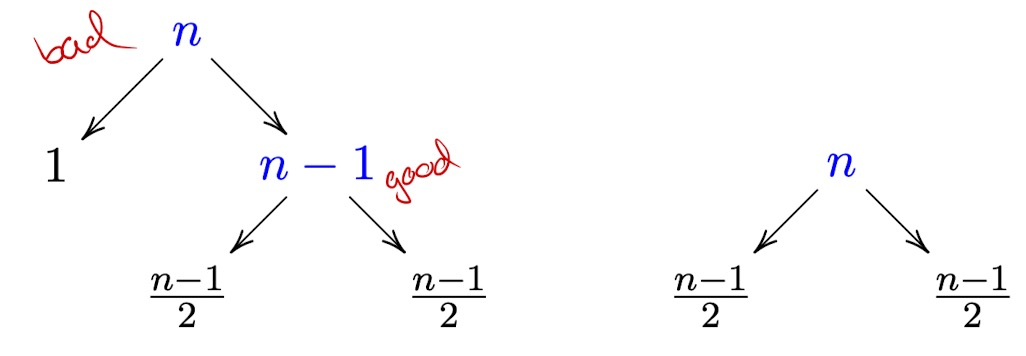
\includegraphics[width=0.5\linewidth]{images/Screenshot 2024-05-30 at 18.21.54.jpg}
    \end{figure}
    \item $G(n)=2B(n/2)+\Theta(n)$ and $B(n)=G(n-1)+\Theta(n)$
     \begin{align*}
        G(n)&=2B(n/2)+\Theta(n)\\
        &=2G(n/2-1)+\Theta(n/2)+\Theta(n)\\
        &=2G(n/2-1)+\Theta \leq 2G(n/2)+\Theta(n)
    \end{align*}
    \item It follows that, on average: $T(n)=\Theta(n \log_2 n)$
    \item Underlying assumption: all permutations of the input numbers are equally likely
    \item Randomized algorithm: partition around random item (instead of last item) 
\end{itemize}



\begin{minipage}{0.55\textwidth} % Adjust the width as needed
\centering % Center the content within the minipage
\begin{algorithm}[H]
\caption{RandomizedHoareParition(A,l,r)}
i = Random(l,r)\;
exchange A[i] and A[r]\;
\textbf{return} HoarePartition(A,l,r)\;
\end{algorithm}
\end{minipage}
\begin{minipage}{0.5\textwidth} % Adjust the width as needed
\centering % Center the content within the minipage
\begin{algorithm}[H]
\caption{RandomizedQuickSort(A,l,r)}
\If{$l<r$}{
m = RandomizedHoarePartition(A,l,r)\;
RandomizedQuickSort(A,l,m-1)\;
RandmoizedQuickSort(A,m,r)\;
}
\end{algorithm}
\end{minipage}


\section{Pointers, Abstract Data Types}
\subsection{Dynamic Data Structures}
Arrays as data structures:
\begin{itemize}
    \item Used to store and manipulate collections of items
    \begin{itemize}
        \item Advantage that one can directly access items
    \end{itemize}
    \item But there are certain limitations or disadvantages
    \begin{itemize}
        \item Dimension of an array is fixed 
        \item Occupies an amount of memory that must be determined beforehand
        \item Inserting/removing items may be expensive operations
    \end{itemize}
    \item A possible solution: Use of dynamic data structures
    \begin{itemize}
        \item Resources are allocated only when they are needed
        \item Items are represented by records/objects whose fields can be accessed if one has a pointer to the object
        \item Change the way in which items are inserted/removed
    \end{itemize}
\end{itemize}

Linked data structures:
\begin{itemize}
    \item Used to deal with collections of items dynamically
    \item Record contains fields that point to other records
    \item Storage space of linked data structures is not known in advance
\end{itemize}

\subsubsection{Pointers}

\textbf{\underline{Pointers in C:}}\\

Operations with pointers:
\begin{itemize}
    \item To follow (chase, dereference) a pointer we write $^*p$ \quad ($ *p = 12$)
    \item To get the address of a variable $i$ we write $\&i$ \quad ($p=\&i$)
    \item To allocate memory we use $malloc(sizeof(Type))$ \quad ($p  = malloc(sizeof(int))$)
    \item To free storage space pointed to by a pointer $p$ we use $free$ \quad ($free(p)$)
\end{itemize}

Declarations of pointers:
\begin{itemize}
    \item To declare a pointer to type T we write $T^*$ \quad ($int* p$)
    \item Note that $^*$ is used for two purposes: 
    \begin{itemize}
        \item Declaring a pointer ($int* p$) and following a pointer $*p=15$
    \end{itemize}
\end{itemize}


\subsubsection{Linked Lists}
\begin{itemize}
    \item A list of integers:
    \begin{figure}[H]
        \centering
        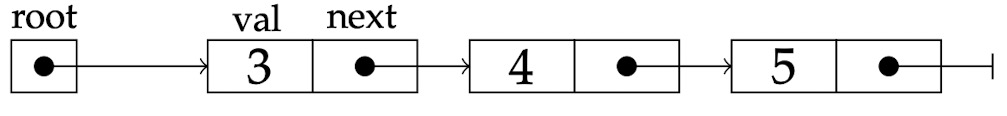
\includegraphics[width=0.5\linewidth]{images/Screenshot 2024-05-30 at 19.03.47.jpg}
    \end{figure}
    \begin{minipage}{0.5\textwidth}
    \item Corresponding declaration in C:
    \begin{lstlisting}
struct node {
    int val;
    struct node* next;
};

struct node* root;
\end{lstlisting}
\end{minipage}
\item Accessing a field: \texttt{p->a}
\end{itemize}
Populating a list with integers:\\

\begin{center}
\begin{minipage}{0.6\textwidth}

\begin{lstlisting}
root = malloc(sizeof(struct node));
root->val = 88;
root->next = malloc(sizeof(struct node));

p = root->next;
p->val = 52;
p->next = malloc(sizeof(struct node));

p = p->next;
p->val = 12;
p->next = NULL;

/* print all elements of a list */
p = root;
while (p != NULL) {
    printf("%d,", p->val);
    p = p->next;
}
printf("\n");
\end{lstlisting}
\end{minipage}
\end{center}

Cost of linked list operations:
\begin{itemize}
    \item Insertion at beginning: $O(1)$
    \item Insert at end: $O(n)$
    \item isEmpty: $O(1)$
    \item Delete: $O(n)$
    \item Print: $O(n)$
\end{itemize}
Previous code fragments for working with the linked list access the list through global variable root => not good
\begin{itemize}
    \item Thus, there can be at most one linked list
    \item The code does not allow us to define and use multiple linked lists
\end{itemize}

Variants of linked lists:
\begin{itemize}
    \item Lists with explicit tail
    \begin{itemize}
        \item Do have an extra pointer to the last item of the list
        \item No need to scan the entire list if an operation applies only to the last item
    \end{itemize}
    \item Doubly linked list
    \begin{itemize}
        \item Each node has a field with a pointer to the previous node of the linked list
        \item Provides means to quickly navigate back and forth in the linked list
    \end{itemize}
\end{itemize}


\subsection{ADT: Abstract Data Types}



\newpage
\section{Appendix: Mathematical Refreshers}
\subsection{Arithmetic Series}
\begin{align}
    \sum_{i=1}^n i= 1+2+\cdots +n = \frac{n(n+1)}{n} \label{ARSeries}
\end{align}

\subsection{Geometric Series}
Given an integer $n_0$ and a real number $0<a \neq 1$:
\begin{align}
    \sum_{i=0}^n a^{i} = 1 + a + a^2 + \cdots +a^n = \frac{1-a^{n+1}}{1-a} \label{GEOSeries}
\end{align}
Given an integer $n_0$ and a real number $|a|<1$:
\begin{align}
    \sum_{i=0}^\infty a^{i} = \frac{1}{1-a}
\end{align}

\subsection{Logarithms and Powers}
\begin{itemize}
    \item $\log_a(bc)=\log_ab+\log_ac$
    \item $\log_ab=\log_c b / \log_c a$
    \item $\log_a b^c = c \log_a b$
    \item $a^m a^n =a^{m+n}$
    \item $a^{mn}=(a^m)^n $
    \item $a^{\log_a b}=b $
    \item $lg b = ldb = \log_2b $
    \item Notation: $\log_ab= ^{a}\log b$
\end{itemize}

\end{document}
